\begin{figure}[!h]
\centering
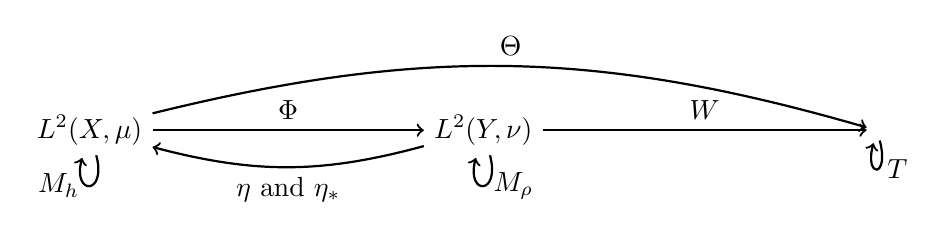
\begin{tikzpicture}[->, thick]
  % Nodes
  \node (A) at (0, 0) {\(L^2(X, \mu)\)};
  \node (B) at (5, 0) {\(L^2(Y, \nu)\)};
  \node (C) at (10, 0) {\(\cH\)};
  % Arrows
  \draw (A) ->  node[above] {\(\Phi\)} (B);
  \draw (B) ->  node[above] {\(W\)} (C);
  \draw (A) to[bend left=15] node[above] {\(\Theta\)} (C);
  % \draw[loop left, min distance=20mm, looseness=8] (A) edge[loop] node[left] {\(M_{h}\)} (A);
  \draw (A) edge[loop below] node[left] {\(M_{h}\)} (A);
  \draw (B) edge[loop below] node[right] {\(M_{\rho}\)} (B);
  \draw (C) edge[loop below] node[right] {\(T\)} (C);
  \draw (B) to[bend left=15] node[below] {\(\eta\) and  \(\eta_*\)} (A);
\end{tikzpicture}
\end{figure}

% \[
% \xymatrix{
%    & \Phi \ar[rrrr] \ar[d] & & & & \mathcal{H} \\
%    M_h \ar@(ul,dl)[] \ar[dr] & L^2(\mathcal{X},\mu') \ar[r]_{\Phi} \ar@/^1pc/[urrrr] & L^2(\mathcal{Y},\nu) \ar[r]^{W} & \mathcal{H} \\
%    & m \ar@/_/[ur] \ar@/_/[rr] & & y^*
% }
% \] 

